
\chapter{The Base Pipeline and its Limits} 
\label{chap:base_pipeline}

This chapter presents the baseline architecture of our embedding pipeline and the related experimental results. The purpose is to detail how the embedding problem was methodologically approached, which embedding optimization methods were selected and tested, and what scalability limitations  and fitness scores emerged. Finally, will be discussed how these limitations are natively imposed by the interplay between the mathematical formulation and the specific hardware constraints of the target quantum platform.

\section{Base pipeline: conceptual scheme}
\label{section:conceptual_base_pipeline}

\begin{figure}[htbp]
    \centering
    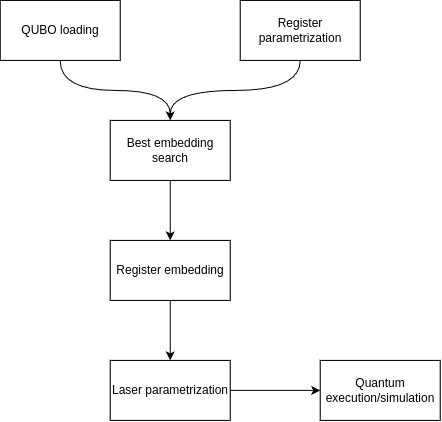
\includegraphics[width=0.5\textwidth]{img/base_pipeline.png} 
    \caption{Flowchart of the basic pipeline. The process highlights an hybrid classical-quantum approach.}
    \label{fig:base_pipeline}
\end{figure}

As illustrated in the conceptual scheme in Figure \ref{fig:base_pipeline}, the first operational phase of the pipeline requires loading the QUBO problem instance. Therefore, it is strictly necessary to detail the geometric and mathematical characteristics of the investigated instances, as well as the hardware restrictions that dictated their generation.

\subsection{Hardware Constraints and the Jülich HPC Emulator}
As discussed, neutral atom platforms present some physical limitations. The most impactful constraint for our formulation is the reliance on a \textit{global driving laser}, which uniformly illuminates the entire atomic register and so imposes the impossibility to excite differently different atoms or clusters of different atoms. Mathematically, this enables a feasible quantum execution only for QUBO matrices that exhibit uniform values on the principal diagonal (representing a constant linear cost/detuning) and uniform off-diagonal penalties (representing the binary Rydberg blockade).

In order to emulate as much as possible a real-world applicability of this thesis, the pipeline was explicitly designed to target \textbf{Jade}, a state-of-the-art Neutral Atom Quantum Processing Unit \cite{pasqal2026italy}. While we initially planned for physical execution on it, access to the actual Jade hardware was postponed to the upcoming December due to broader availability constraints. Consequently, the experimental phase for the moment has relied to a remote analog quantum emulator provided by the \textbf{Jülich Supercomputing Centre (JSC)} in Germany. 

To ensure that the research performed remains perfectly forward-compatible with the real machine once available, we injected a custom hardware profile into the simulator (referred to in the codebase \cite{orsucci_qubo_ga_quantum} as \texttt{FakeJade}). This profile strictly enforces Jade's actual physical parameters in order to be able to directly test this work on it in the near future.


The \texttt{FakeJade} physical profile injected into the emulator severely bounds the degrees of freedom available to the classical embedding algorithm. Extracting directly from platform API call, the hardware constraints are the following:

\begin{itemize}
    \item \textbf{Maximum Radius ($R_{max}$):} The entire atomic register must be confined within a specific continuous area dictated by the laser focusing limits. For our emulator, the coordinates confined within a circular plane with a maximum radius of $R_{max} = 50.0\,\mu\text{m}$.
    
    \item \textbf{Minimum atomic distance ($d_{min}$):} Due to the diffraction limits of the optical tweezers, two atoms cannot be placed arbitrarily close or overlapped (we are considering a 2D register). The hardware enforces a minimum inter-atomic distance of $d_{min} = 4.0\,\mu\text{m}$. Breaching this threshold causes a hard physical violation and the impossibility to submit the task to remote infrastructure.
    
    \item \textbf{Interaction Saturation ($V_{max}$):} Neutral atoms interact following the Van der Waals potential ($V = C_6 / r^6$), the combination of physical laws and the $d_{min}$ constraint, caps the maximum possible interaction strength between any two qubits. The highest tolerable penalty in the system is saturated at $V_{max} = C_6 / d_{min}^6$.
    
    \item \textbf{Global Channel Energetics and Scaling:} The QPU operates via a single \texttt{rydberg\_global} channel. This imposes ceilings on the maximum allowable Rabi frequency ($\Omega_{max}$) and the maximum absolute detuning ($|\delta|_{max}$). Because raw QUBO weights can mathematically exceed these physical capacities, the embedding pipeline must calculate a restrictive \textit{Scale Factor}. As implemented in the codebase \cite{orsucci_qubo_ga_quantum}, the entire QUBO matrix is dynamically (instance per instance) scaled down by a factor of $\min(\frac{V_{max}}{\max(Q_{off-diagonal})}, \frac{|\delta|_{max}}{\text{avg}(Q_{diagonal})})$ to ensure the problem fits within the hardware's physical energy envelope.
\end{itemize}

\subsection{QUBO Instance Generation}
These strict hardware parameters played a foundational role in how the test datasets were generated. To guarantee that the problem instances are physically embeddable on the targeted neutral atom architecture, a specialized Python generation script was developed. Rather than generating arbitrary random graphs, the script synthesizes ``verisimilar'' Unit Disk Graphs (UDG) by simulating the actual physical placement of atoms under the constraints aforementioned.
The generation logic is composed by the following procedural steps:
\begin{enumerate}
    \item \textbf{Dynamic Operational Area Calculation:} To achieve a specific target average degree (which dictates primarly the problem's difficulty), an effective operational radius is dynamically calculated. This radius scales proportionally with the square root of the number of nodes ($N$) and the Rydberg radius. Most important, it is mathematically bounded to never exceed the physical limits of the machine (the $50\,\mu\text{m}$ maximum hardware radius) while remaining large enough to accommodate all atoms.
    \item \textbf{Rejection Sampling Placement:} Node coordinates are generated uniformly within the operational area using polar coordinates. An hardware aware minimum-distance check is enforced during this process: any randomly generated position that falls within the minimum allowed optical trap distance ($d_{min} = 4.0\,\mu\text{m}$) of an already placed atom is immediately rejected. This ensures the resulting spatial configuration respects the optical tweezers' constraints.
    \item \textbf{QUBO Matrix Construction:} Once all $N$ coordinates are successfully placed within the delimited continuous space, the pairwise Euclidean distance matrix is computed. The QUBO matrix ($Q$) is then populated: all main diagonal elements are uniformly set to $-1.0$ (representing the global laser's tendency to drive the atoms toward the Rydberg state), and a constant penalty weight of $2.0$ is assigned to any off-diagonal edge where the inter-atomic distance is strictly less than the specified Rydberg blockade radius set ($R_b = 12.0\,\mu\text{m}$).
    \item \textbf{Data Serialization:} Finally, the non-zero upper triangular elements of the QUBO matrix are extracted and serialized into a (\texttt{.npz}) format. Although the original geometrically valid coordinates are stored for validation purposes, the embedding pipeline receives only the abstract mathematical weights (otherwise all of the next experimentations do not makes much sense), forcing the selected embedding algorithm to reconstruct a valid physical layout from scratch.
\end{enumerate}

\begin{figure}[htbp]
    \centering
    
     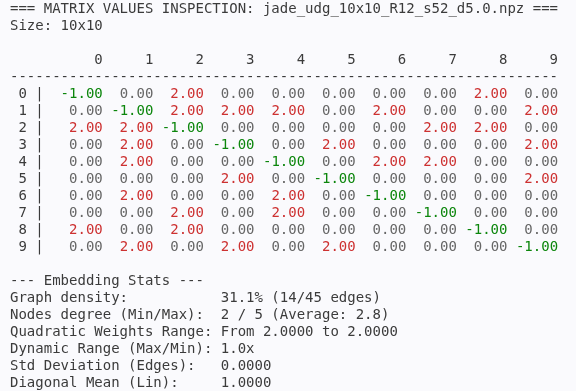
\includegraphics[width=0.6\textwidth]{img/QUBO_example.png} 
    \caption{Example of a small-scale UDG-like QUBO instance generated using the \textit{instance\_generator.py} as described above and inspected via \textit{inspect\_qubo.py} in \cite{orsucci_qubo_ga_quantum}.}
    \label{fig:qubo_generation_example}
\end{figure}

\subsection{Instance Loading and Matrix Parsing}
Once generated, the QUBO matrices and their metadata are compressed and stored in NumPy's binary format (\texttt{.npz}). As depicted in the first block of the pipeline flowchart, the execution begins with the \texttt{QUBO loading} module. 

A dedicated parser function extracts the indices and weights from the \texttt{.npz} file and reconstructs the symmetric $N \times N$ matrix ($Q$). Simultaneously, the system isolates the off-diagonal terms to calculate the maximum theoretical connectivity. 

\section{Embedding Optimization using Genetic Algorithms (GA)}
\label{sec:ga_optimization}

The search for an optimal physical embedding is a $NP$-Hard task characterized by a highly complex, non-convex optimization scenario that makes very ineffective using classical optimization methods such as the Nelder-Mead simplex method. As formalized in the previous section, among the challenges, we have that the computational engine must simultaneously satisfy strict geometric boundaries ($R_{max}$) and discrete proximity constraints ($d_{min}$) for example, all while minimizing in some way the topological error between the physical Van der Waals interactions and the mathematical QUBO penalties in order
to achieve a good enough fitness score and consequently (at least in principal) a good enough embedding.

Given the severity of these constraints and the complete lack of \textit{a priori} analytical information regarding the optimal spatial distribution of the atoms, we choose to initiate our experimental phase by testing a black-box, derivative-free optimization approach: Genetic Algorithms (GAs). This section has the main goal
to explain the main GAs' characteristics finalized to better contextualize the more attentioned experimental results.  


%ancora da ricontrollare
\paragraph{Genetic Algorithm Framework}
Genetic Algorithms represent a prominent branch of evolutionary computation, heavily inspired by the biological principles of natural selection and genetics. The possible different methodological classifications and terminologies are very different and influenced by the different biological and evolutionary elements inspiring the different algorithms, 
but in general they are particularly well-suited for optimization problems where the search space is discontinuous and when we don't have a priori information at all.

In our specific context of application, as a result of deep and complete study of \cite{bookGA}, considered the bible for Genetic Algorithms, we decided to design our GA with the following key aspects: 

\begin{itemize}
    \item an individual or chromosome in the GA population is a set of 2 continue 2D coordinates $(x,y)$ having a 2D register. A set for every $N$ atoms (binary variables).
    \item the population is iteratevely improved via crossover, parenting, selection...
    \item the population evalutation and improvement is done using a fitness function score as metric.
\end{itemize}

%continuare con esempio di configurazione GA
%spiegare nel dettaglio perchè è stata fatta questa scelta
%spiegare con esempio la fitness function, formalizzarla e spiegare perchè è stata scelta.